\documentclass[]{book}
\usepackage{lmodern}
\usepackage{amssymb,amsmath}
\usepackage{ifxetex,ifluatex}
\usepackage{fixltx2e} % provides \textsubscript
\ifnum 0\ifxetex 1\fi\ifluatex 1\fi=0 % if pdftex
  \usepackage[T1]{fontenc}
  \usepackage[utf8]{inputenc}
\else % if luatex or xelatex
  \ifxetex
    \usepackage{mathspec}
  \else
    \usepackage{fontspec}
  \fi
  \defaultfontfeatures{Ligatures=TeX,Scale=MatchLowercase}
\fi
% use upquote if available, for straight quotes in verbatim environments
\IfFileExists{upquote.sty}{\usepackage{upquote}}{}
% use microtype if available
\IfFileExists{microtype.sty}{%
\usepackage[]{microtype}
\UseMicrotypeSet[protrusion]{basicmath} % disable protrusion for tt fonts
}{}
\PassOptionsToPackage{hyphens}{url} % url is loaded by hyperref
\usepackage[unicode=true]{hyperref}
\hypersetup{
            pdftitle={Merck-Data Mine Documentation},
            pdfauthor={Merck and Data Mine Corporate Partnership Team},
            pdfborder={0 0 0},
            breaklinks=true}
\urlstyle{same}  % don't use monospace font for urls
\usepackage{natbib}
\bibliographystyle{apalike}
\usepackage{color}
\usepackage{fancyvrb}
\newcommand{\VerbBar}{|}
\newcommand{\VERB}{\Verb[commandchars=\\\{\}]}
\DefineVerbatimEnvironment{Highlighting}{Verbatim}{commandchars=\\\{\}}
% Add ',fontsize=\small' for more characters per line
\usepackage{framed}
\definecolor{shadecolor}{RGB}{248,248,248}
\newenvironment{Shaded}{\begin{snugshade}}{\end{snugshade}}
\newcommand{\KeywordTok}[1]{\textcolor[rgb]{0.13,0.29,0.53}{\textbf{#1}}}
\newcommand{\DataTypeTok}[1]{\textcolor[rgb]{0.13,0.29,0.53}{#1}}
\newcommand{\DecValTok}[1]{\textcolor[rgb]{0.00,0.00,0.81}{#1}}
\newcommand{\BaseNTok}[1]{\textcolor[rgb]{0.00,0.00,0.81}{#1}}
\newcommand{\FloatTok}[1]{\textcolor[rgb]{0.00,0.00,0.81}{#1}}
\newcommand{\ConstantTok}[1]{\textcolor[rgb]{0.00,0.00,0.00}{#1}}
\newcommand{\CharTok}[1]{\textcolor[rgb]{0.31,0.60,0.02}{#1}}
\newcommand{\SpecialCharTok}[1]{\textcolor[rgb]{0.00,0.00,0.00}{#1}}
\newcommand{\StringTok}[1]{\textcolor[rgb]{0.31,0.60,0.02}{#1}}
\newcommand{\VerbatimStringTok}[1]{\textcolor[rgb]{0.31,0.60,0.02}{#1}}
\newcommand{\SpecialStringTok}[1]{\textcolor[rgb]{0.31,0.60,0.02}{#1}}
\newcommand{\ImportTok}[1]{#1}
\newcommand{\CommentTok}[1]{\textcolor[rgb]{0.56,0.35,0.01}{\textit{#1}}}
\newcommand{\DocumentationTok}[1]{\textcolor[rgb]{0.56,0.35,0.01}{\textbf{\textit{#1}}}}
\newcommand{\AnnotationTok}[1]{\textcolor[rgb]{0.56,0.35,0.01}{\textbf{\textit{#1}}}}
\newcommand{\CommentVarTok}[1]{\textcolor[rgb]{0.56,0.35,0.01}{\textbf{\textit{#1}}}}
\newcommand{\OtherTok}[1]{\textcolor[rgb]{0.56,0.35,0.01}{#1}}
\newcommand{\FunctionTok}[1]{\textcolor[rgb]{0.00,0.00,0.00}{#1}}
\newcommand{\VariableTok}[1]{\textcolor[rgb]{0.00,0.00,0.00}{#1}}
\newcommand{\ControlFlowTok}[1]{\textcolor[rgb]{0.13,0.29,0.53}{\textbf{#1}}}
\newcommand{\OperatorTok}[1]{\textcolor[rgb]{0.81,0.36,0.00}{\textbf{#1}}}
\newcommand{\BuiltInTok}[1]{#1}
\newcommand{\ExtensionTok}[1]{#1}
\newcommand{\PreprocessorTok}[1]{\textcolor[rgb]{0.56,0.35,0.01}{\textit{#1}}}
\newcommand{\AttributeTok}[1]{\textcolor[rgb]{0.77,0.63,0.00}{#1}}
\newcommand{\RegionMarkerTok}[1]{#1}
\newcommand{\InformationTok}[1]{\textcolor[rgb]{0.56,0.35,0.01}{\textbf{\textit{#1}}}}
\newcommand{\WarningTok}[1]{\textcolor[rgb]{0.56,0.35,0.01}{\textbf{\textit{#1}}}}
\newcommand{\AlertTok}[1]{\textcolor[rgb]{0.94,0.16,0.16}{#1}}
\newcommand{\ErrorTok}[1]{\textcolor[rgb]{0.64,0.00,0.00}{\textbf{#1}}}
\newcommand{\NormalTok}[1]{#1}
\usepackage{longtable,booktabs}
% Fix footnotes in tables (requires footnote package)
\IfFileExists{footnote.sty}{\usepackage{footnote}\makesavenoteenv{long table}}{}
\usepackage{graphicx,grffile}
\makeatletter
\def\maxwidth{\ifdim\Gin@nat@width>\linewidth\linewidth\else\Gin@nat@width\fi}
\def\maxheight{\ifdim\Gin@nat@height>\textheight\textheight\else\Gin@nat@height\fi}
\makeatother
% Scale images if necessary, so that they will not overflow the page
% margins by default, and it is still possible to overwrite the defaults
% using explicit options in \includegraphics[width, height, ...]{}
\setkeys{Gin}{width=\maxwidth,height=\maxheight,keepaspectratio}
\usepackage[normalem]{ulem}
% avoid problems with \sout in headers with hyperref:
\pdfstringdefDisableCommands{\renewcommand{\sout}{}}
\IfFileExists{parskip.sty}{%
\usepackage{parskip}
}{% else
\setlength{\parindent}{0pt}
\setlength{\parskip}{6pt plus 2pt minus 1pt}
}
\setlength{\emergencystretch}{3em}  % prevent overfull lines
\providecommand{\tightlist}{%
  \setlength{\itemsep}{0pt}\setlength{\parskip}{0pt}}
\setcounter{secnumdepth}{5}
% Redefines (sub)paragraphs to behave more like sections
\ifx\paragraph\undefined\else
\let\oldparagraph\paragraph
\renewcommand{\paragraph}[1]{\oldparagraph{#1}\mbox{}}
\fi
\ifx\subparagraph\undefined\else
\let\oldsubparagraph\subparagraph
\renewcommand{\subparagraph}[1]{\oldsubparagraph{#1}\mbox{}}
\fi

% set default figure placement to htbp
\makeatletter
\def\fps@figure{htbp}
\makeatother

\usepackage{booktabs}
\usepackage{amsthm}
\makeatletter
\def\thm@space@setup{%
  \thm@preskip=8pt plus 2pt minus 4pt
  \thm@postskip=\thm@preskip
}
\makeatother

\title{Merck-Data Mine Documentation}
\author{Merck and Data Mine Corporate Partnership Team}
\date{2020-09-23}

\begin{document}
\maketitle

{
\setcounter{tocdepth}{1}
\tableofcontents
}
\chapter{Introduction}\label{introduction}

This book will serve as tutorial based documentation for the Merck -
Data Mine Coporate Partnership team for the 2020-2021 academic year.

\section{How to contribute}\label{how-to-contribute}

Contributing to this book is simple:

\subsection{Larger changes or
additions}\label{larger-changes-or-additions}

If you have larger changes or additions you'd like to make to the book,
the easiest way is to edit the contents of the book on your local
machine.

\subsubsection{\texorpdfstring{Using \texttt{git} in the
terminal}{Using git in the terminal}}\label{using-git-in-the-terminal}

\begin{enumerate}
\def\labelenumi{\arabic{enumi}.}
\tightlist
\item
  Setup \texttt{git} following the directions
  \protect\hyperlink{git-install}{here}.
\item
  Start by opening up a terminal and
  \protect\hyperlink{configure-git}{configuring \texttt{git} to work
  with GitHub}.
\item
  Navigate to the directory in which you would like to clone
  the-examples-book repository. For example, if I wanted to clone the
  repository in my \texttt{\textasciitilde{}/projects} folder, I'd first
  execute: \texttt{cd\ \textasciitilde{}/projects}.
\item
  \protect\hyperlink{git-clone-repository}{Clone the repository}. In
  this example, let's assume I've cloned the repository into my
  \texttt{\textasciitilde{}/projects} folder.
\item
  Navigate into the project folder:
\end{enumerate}

\begin{Shaded}
\begin{Highlighting}[]
\BuiltInTok{cd}\NormalTok{ ~/projects/the-examples-book}
\end{Highlighting}
\end{Shaded}

\begin{enumerate}
\def\labelenumi{\arabic{enumi}.}
\setcounter{enumi}{5}
\tightlist
\item
  At this point in time your current branch should be the
  \texttt{master} branch. You can verify by running:
\end{enumerate}

\begin{Shaded}
\begin{Highlighting}[]
\FunctionTok{git}\NormalTok{ branch}
\end{Highlighting}
\end{Shaded}

\textbf{Note:} The highlighted branch starting with ``*" is the current
branch.

or if you'd like just the name of the branch:

\begin{Shaded}
\begin{Highlighting}[]
\FunctionTok{git}\NormalTok{ rev-parse --abbrev-ref HEAD}
\end{Highlighting}
\end{Shaded}

\begin{enumerate}
\def\labelenumi{\arabic{enumi}.}
\setcounter{enumi}{6}
\item
  \protect\hyperlink{git-create-new-branch}{Create a new branch} with
  whatever name you'd like, and check that branch out. For example,
  \texttt{fix-spelling-errors-01}.
\item
  Open up RStudio. In the ``Files'' tab in RStudio, navigate to the
  repository. In this example, we would navigate to
  \texttt{/Users/kamstut/Documents/GitHub/the-examples-book}. Click on
  the ``More'' dropdown and select ``Set As Working Directory''.
\item
  If you do not already have \texttt{renv} installed, install it by
  running the following commands in the console:
\end{enumerate}

\begin{Shaded}
\begin{Highlighting}[]
\KeywordTok{install.packages}\NormalTok{(}\StringTok{"renv"}\NormalTok{)}
\end{Highlighting}
\end{Shaded}

\begin{enumerate}
\def\labelenumi{\arabic{enumi}.}
\setcounter{enumi}{9}
\tightlist
\item
  Restore the environment by running the following commands in the
  console:
\end{enumerate}

\begin{Shaded}
\begin{Highlighting}[]
\NormalTok{renv}\OperatorTok{::}\KeywordTok{restore}\NormalTok{()}
\end{Highlighting}
\end{Shaded}

\begin{enumerate}
\def\labelenumi{\arabic{enumi}.}
\setcounter{enumi}{10}
\tightlist
\item
  In order to compile this book, you must have LaTeX installed. The
  easiest way to accomplish this is to run the following in the R
  console:
\end{enumerate}

\begin{Shaded}
\begin{Highlighting}[]
\KeywordTok{install.packages}\NormalTok{(}\StringTok{"tinytex"}\NormalTok{)}
\KeywordTok{library}\NormalTok{(tinytex)}
\NormalTok{tinytex}\OperatorTok{::}\KeywordTok{install_tinytex}\NormalTok{()}
\end{Highlighting}
\end{Shaded}

\begin{enumerate}
\def\labelenumi{\arabic{enumi}.}
\setcounter{enumi}{11}
\item
  In addition, make sure to install both \texttt{pandoc} and
  \texttt{pandoc-citeproc} by following the instructions
  \href{https://pandoc.org/installing.html}{here}.
\item
  Modify the \texttt{.Rmd} files to your liking.
\item
  Click the ``Knit'' button to compile the book. The resulting ``book''
  is within the ``docs'' folder.
\end{enumerate}

\textbf{Important note:} If at any point in time you receive an error
saying something similar to ``there is no package called
\texttt{my\_package}, simply install the missing package, and try to
knit again:

\begin{Shaded}
\begin{Highlighting}[]
\KeywordTok{install.packages}\NormalTok{(}\StringTok{"my_package"}\NormalTok{)}
\KeywordTok{library}\NormalTok{(my_package)}
\end{Highlighting}
\end{Shaded}

\begin{enumerate}
\def\labelenumi{\arabic{enumi}.}
\setcounter{enumi}{14}
\tightlist
\item
  To test the book out, navigate to the ``docs'' folder and open the
  \texttt{index.html} in the browser of your choice.
\item
  When you are happy with the modifications you've made,
  \protect\hyperlink{git-commit-changes}{commit your changes} to the
  repository.
\item
  You can continue to make modifications and commit your changes
  locally. When you are ready, you can
  \protect\hyperlink{git-push-local-commits}{push your branch} to the
  remote repository (github.com).
\item
  At this point in time, you can confirm that the branch has been
  succesfully pushed to github.com by navigating to the repository on
  github, and click on the ``branches'' tab:
\end{enumerate}

\begin{figure}
\centering
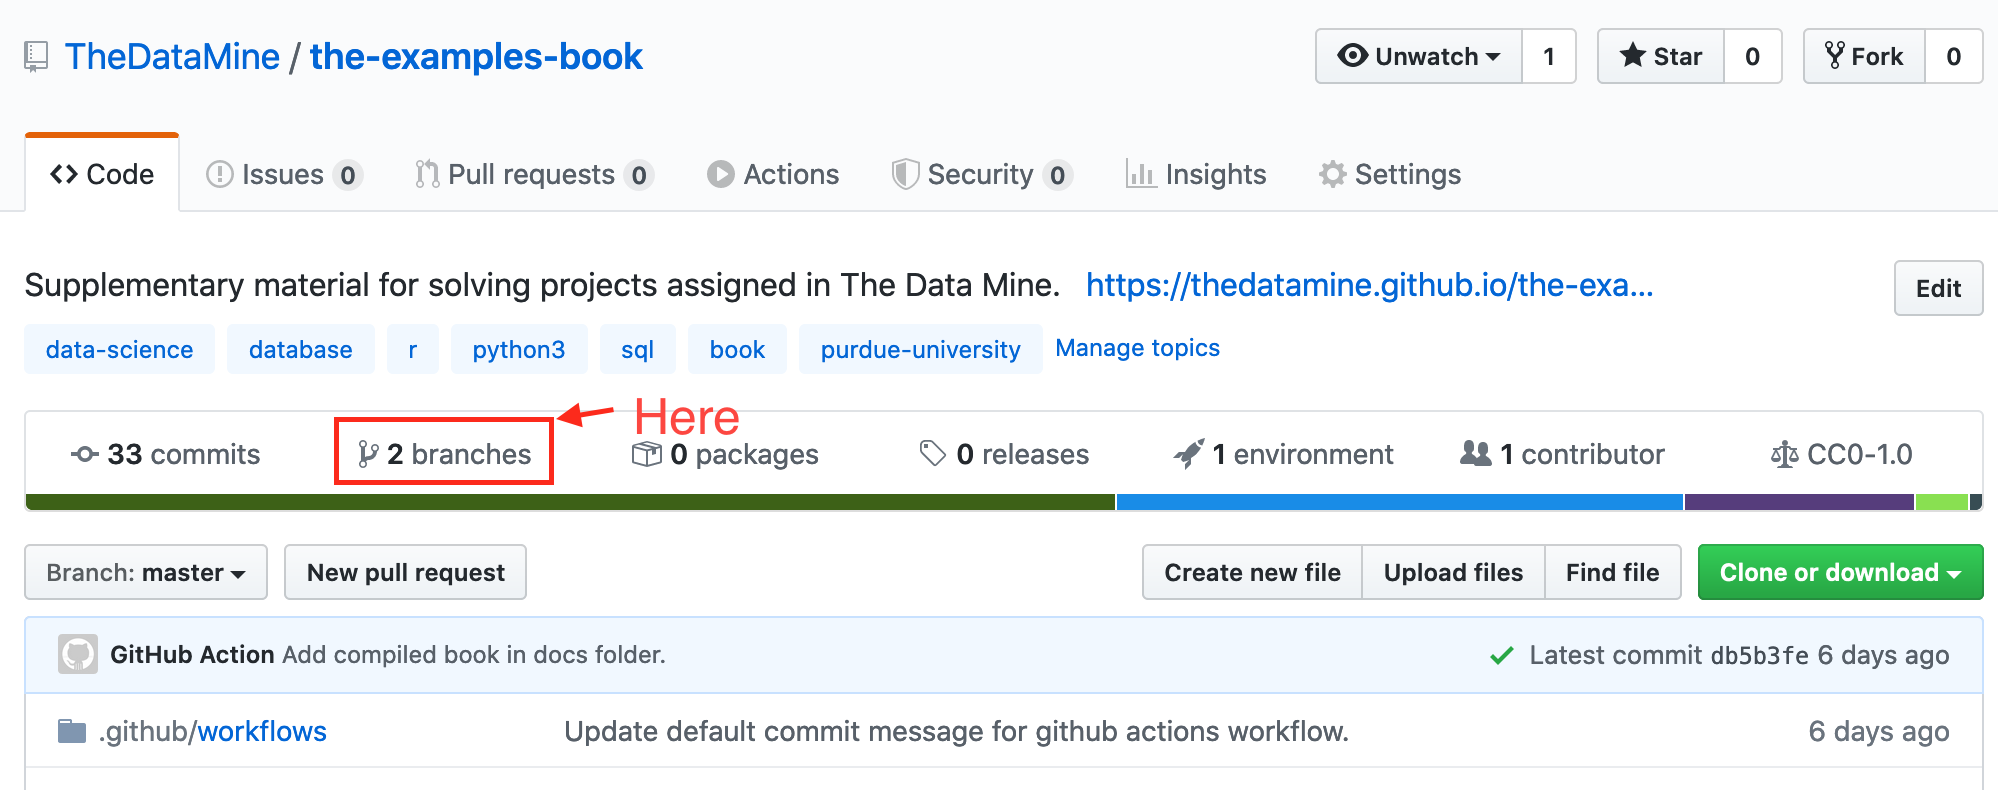
\includegraphics{./images/gh-desktop-14.png}
\caption{}
\end{figure}

\begin{enumerate}
\def\labelenumi{\arabic{enumi}.}
\setcounter{enumi}{18}
\tightlist
\item
  Next, \href{}{create a pull request}. Note that a ``Pull Request'' is
  a GitHub-specific concept. You cannot create a pull request using
  \texttt{git}. Navigate to the repository
  \url{https://github.com/thedatamine/the-examples-book}, and you should
  see a message asking if you'd like to create a pull request:
\end{enumerate}

\begin{figure}
\centering
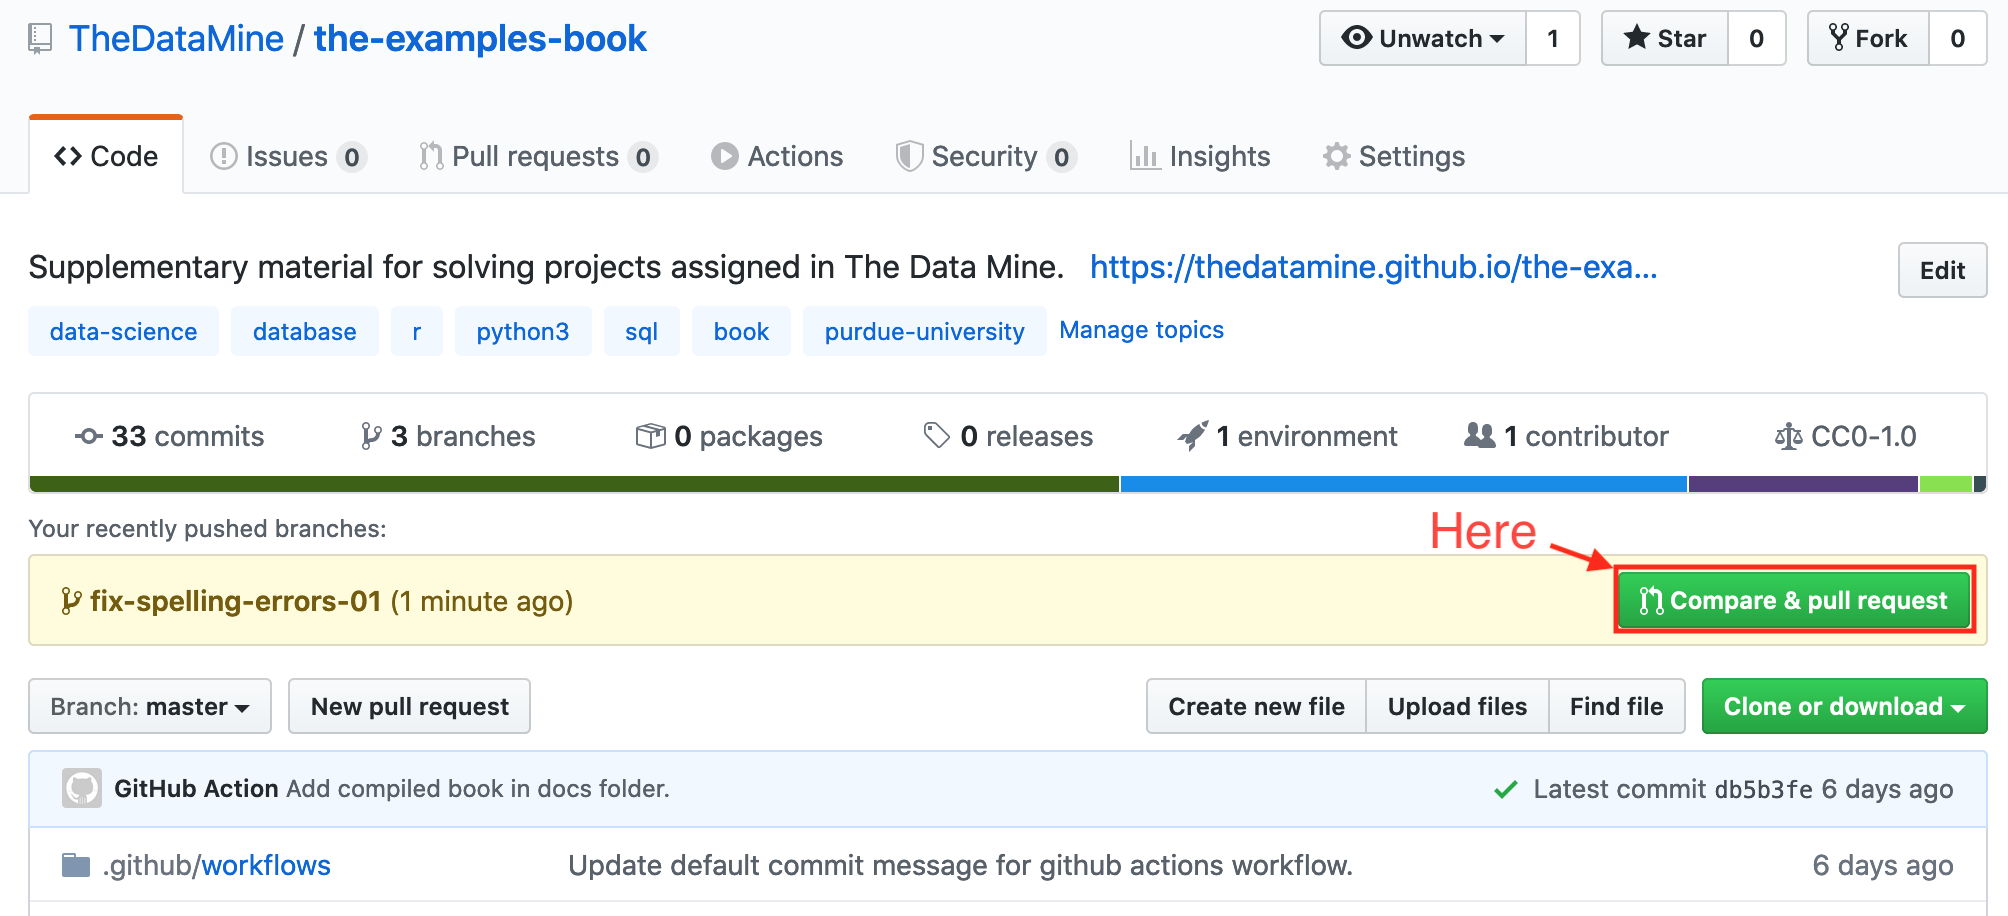
\includegraphics{./images/pr-01.png}
\caption{}
\end{figure}

\begin{enumerate}
\def\labelenumi{\arabic{enumi}.}
\setcounter{enumi}{19}
\item
  Leave a detailed comment about what you've modified or added to the
  book. You can click on ``Preview'' to see what your comment will look
  like.
  \href{https://help.github.com/en/github/writing-on-github/basic-writing-and-formatting-syntax}{GitHub's
  markdown} applies here. Once satisfied, click ``Create pull request''.
\item
  At this point in time, the repository owners will receive a
  notification and will check and potentially merge the changes into the
  \texttt{master} branch.
\end{enumerate}

\subsubsection{Using GitHub Desktop}\label{using-github-desktop}

\begin{enumerate}
\def\labelenumi{\arabic{enumi}.}
\tightlist
\item
  Setup GitHub Desktop following the directions
  \protect\hyperlink{github-desktop-install}{here}.
\item
  When you are presented with the following screen, select ``Clone a
  Repository from the Internet\ldots{}'':
\end{enumerate}

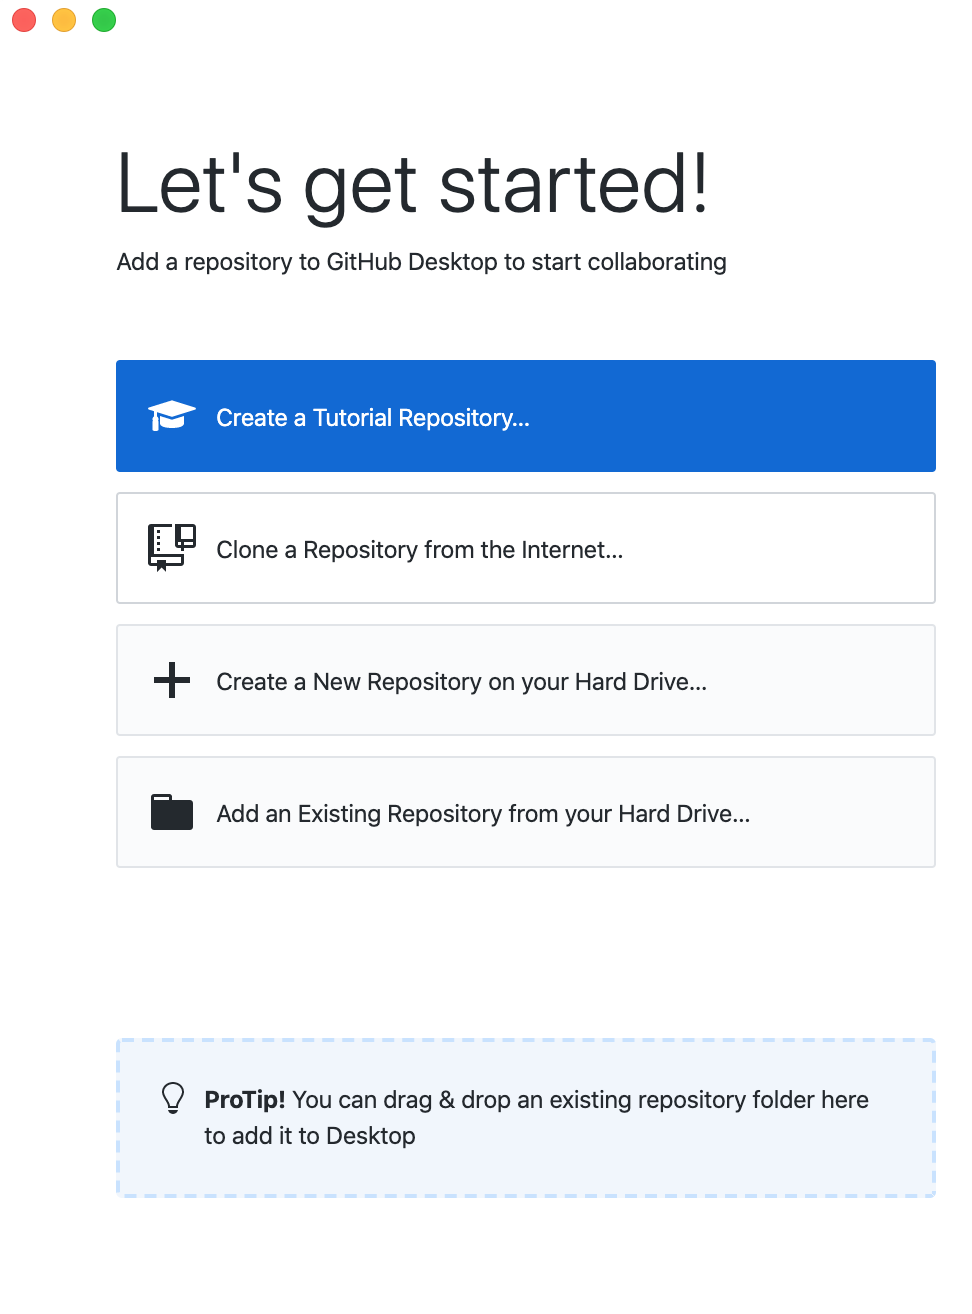
\includegraphics{./images/gh-desktop-03.png} 3. Click on the ``URL''
tab:

\begin{figure}
\centering
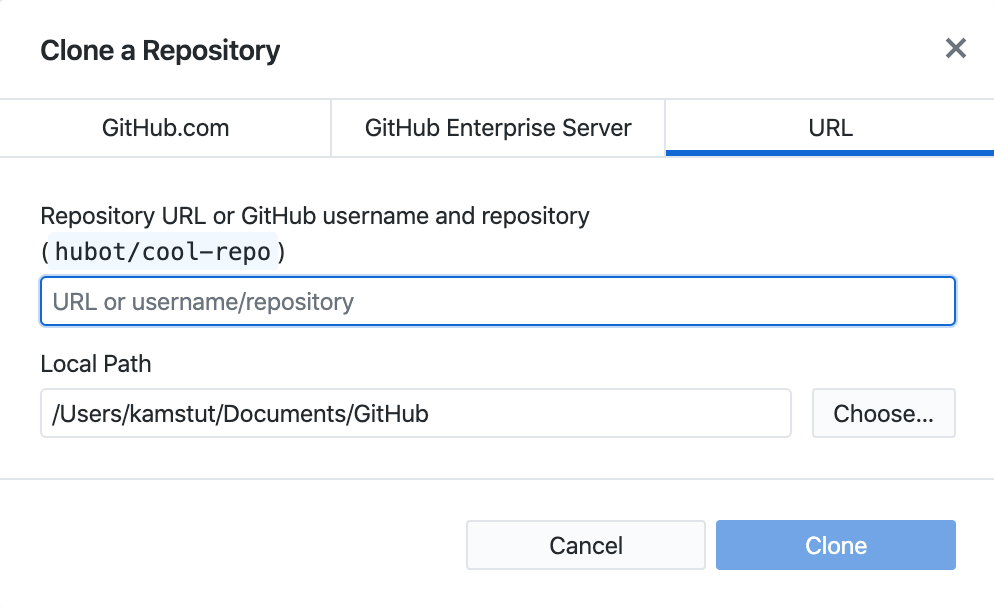
\includegraphics{./images/gh-desktop-04.png}
\caption{}
\end{figure}

\begin{enumerate}
\def\labelenumi{\arabic{enumi}.}
\setcounter{enumi}{3}
\tightlist
\item
  In the first field, enter ``TheDataMine/the-examples-book''. This is
  the repository for this book.
\item
  In the second field, enter the location in which you'd like the
  repository to be cloned to. In this example, the repository will be
  cloned into \texttt{/Users/kamstut/Documents/GitHub}. The result will
  be a new folder called \texttt{the-examples-book} in
  \texttt{/Users/kamstut/Documents/GitHub}.
\item
  Click ``Clone''.
\item
  Upon completion, you will be presented with a screen similar to this:
\end{enumerate}

\begin{figure}
\centering
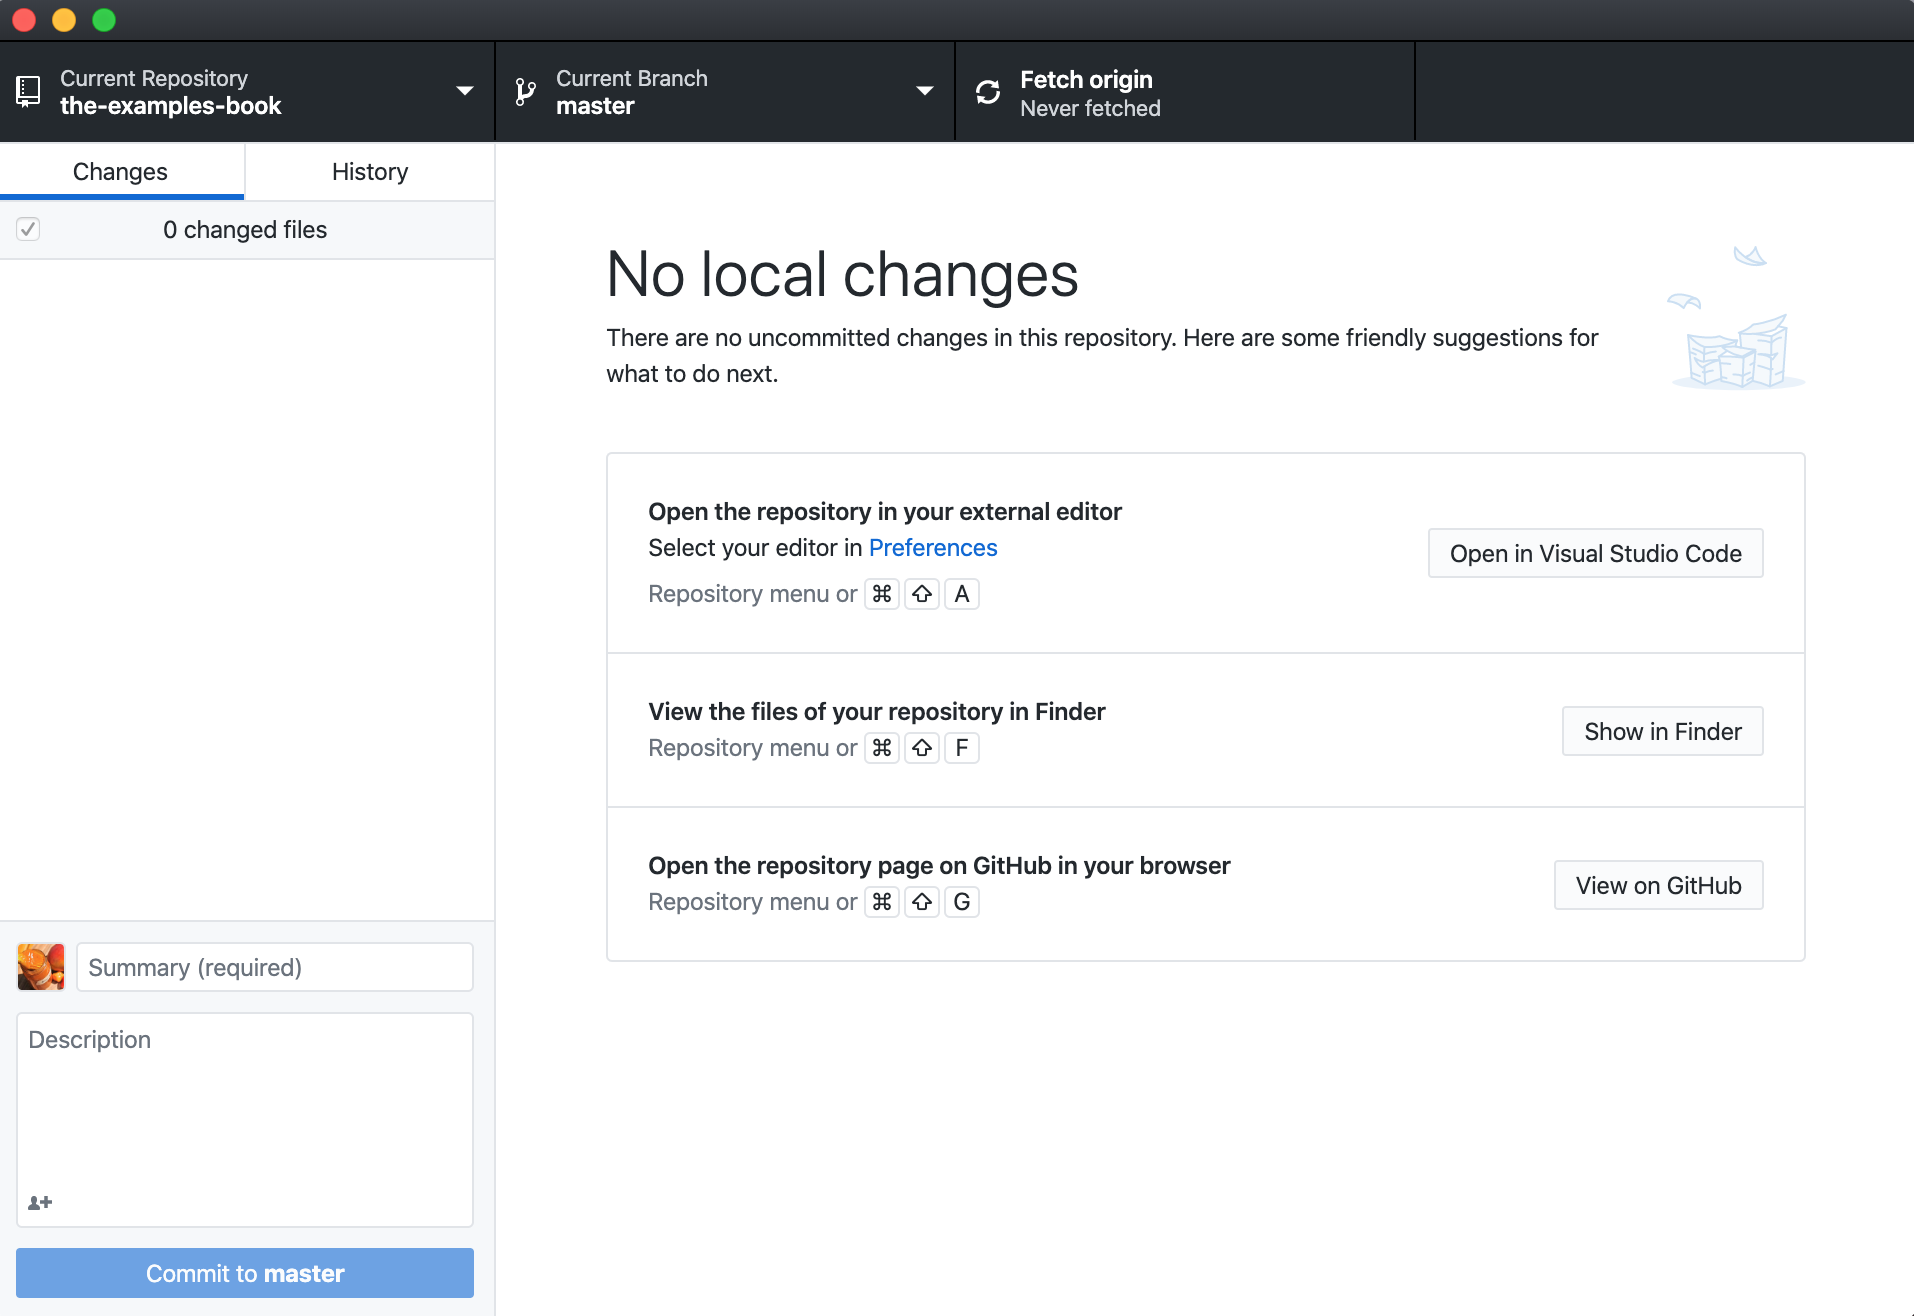
\includegraphics{./images/gh-desktop-05.png}
\caption{}
\end{figure}

\begin{enumerate}
\def\labelenumi{\arabic{enumi}.}
\setcounter{enumi}{7}
\tightlist
\item
  At this point in time, your current branch will be the \texttt{master}
  branch. \protect\hyperlink{github-desktop-create-new-branch}{Create a
  new branch} with whatever name you'd like. For example,
  \texttt{fix-spelling-errors-01}.
\item
  Open up RStudio. In the ``Files'' tab in RStudio, navigate to the
  repository. In this example, we would navigate to
  \texttt{/Users/kamstut/Documents/GitHub/the-examples-book}. Click on
  the ``More'' dropdown and select ``Set As Working Directory''.
\item
  If you do not already have \texttt{renv} installed, install it by
  running the following commands in the console:
\end{enumerate}

\begin{Shaded}
\begin{Highlighting}[]
\KeywordTok{install.packages}\NormalTok{(}\StringTok{"renv"}\NormalTok{)}
\end{Highlighting}
\end{Shaded}

\begin{enumerate}
\def\labelenumi{\arabic{enumi}.}
\setcounter{enumi}{10}
\tightlist
\item
  Restore the environment by running the following commands in the
  console:
\end{enumerate}

\begin{Shaded}
\begin{Highlighting}[]
\NormalTok{renv}\OperatorTok{::}\KeywordTok{restore}\NormalTok{()}
\end{Highlighting}
\end{Shaded}

\begin{enumerate}
\def\labelenumi{\arabic{enumi}.}
\setcounter{enumi}{11}
\tightlist
\item
  In order to compile this book, you must have LaTeX installed. The
  easiest way to accomplish this is to run the following in the R
  console:
\end{enumerate}

\begin{Shaded}
\begin{Highlighting}[]
\KeywordTok{install.packages}\NormalTok{(}\StringTok{"tinytex"}\NormalTok{)}
\KeywordTok{library}\NormalTok{(tinytex)}
\NormalTok{tinytex}\OperatorTok{::}\KeywordTok{install_tinytex}\NormalTok{()}
\end{Highlighting}
\end{Shaded}

\begin{enumerate}
\def\labelenumi{\arabic{enumi}.}
\setcounter{enumi}{12}
\item
  In addition, make sure to install both \texttt{pandoc} and
  \texttt{pandoc-citeproc} by following the instructions
  \href{https://pandoc.org/installing.html}{here}.
\item
  Modify the \texttt{.Rmd} files to your liking.
\item
  Click the ``Knit'' button to compile the book. The resulting ``book''
  is within the ``docs'' folder.
\end{enumerate}

\textbf{Important note:} If at any point in time you receive an error
saying something similar to ``there is no package called
\texttt{my\_package}, simply install the missing package, and try to
knit again:

\begin{Shaded}
\begin{Highlighting}[]
\KeywordTok{install.packages}\NormalTok{(}\StringTok{"my_package"}\NormalTok{)}
\KeywordTok{library}\NormalTok{(my_package)}
\end{Highlighting}
\end{Shaded}

\begin{enumerate}
\def\labelenumi{\arabic{enumi}.}
\setcounter{enumi}{15}
\tightlist
\item
  To test the book out, navigate to the ``docs'' folder and open the
  \texttt{index.html} in the browser of your choice.
\item
  When you are happy with the modifications you've made,
  \protect\hyperlink{github-desktop-commit-changes}{commit your changes}
  to the repository.
\item
  You can continue to make modifications and commit your changes
  locally. When you are ready, you can
  \protect\hyperlink{github-desktop-publish-branch}{publish your
  branch}:
\end{enumerate}

\begin{figure}
\centering
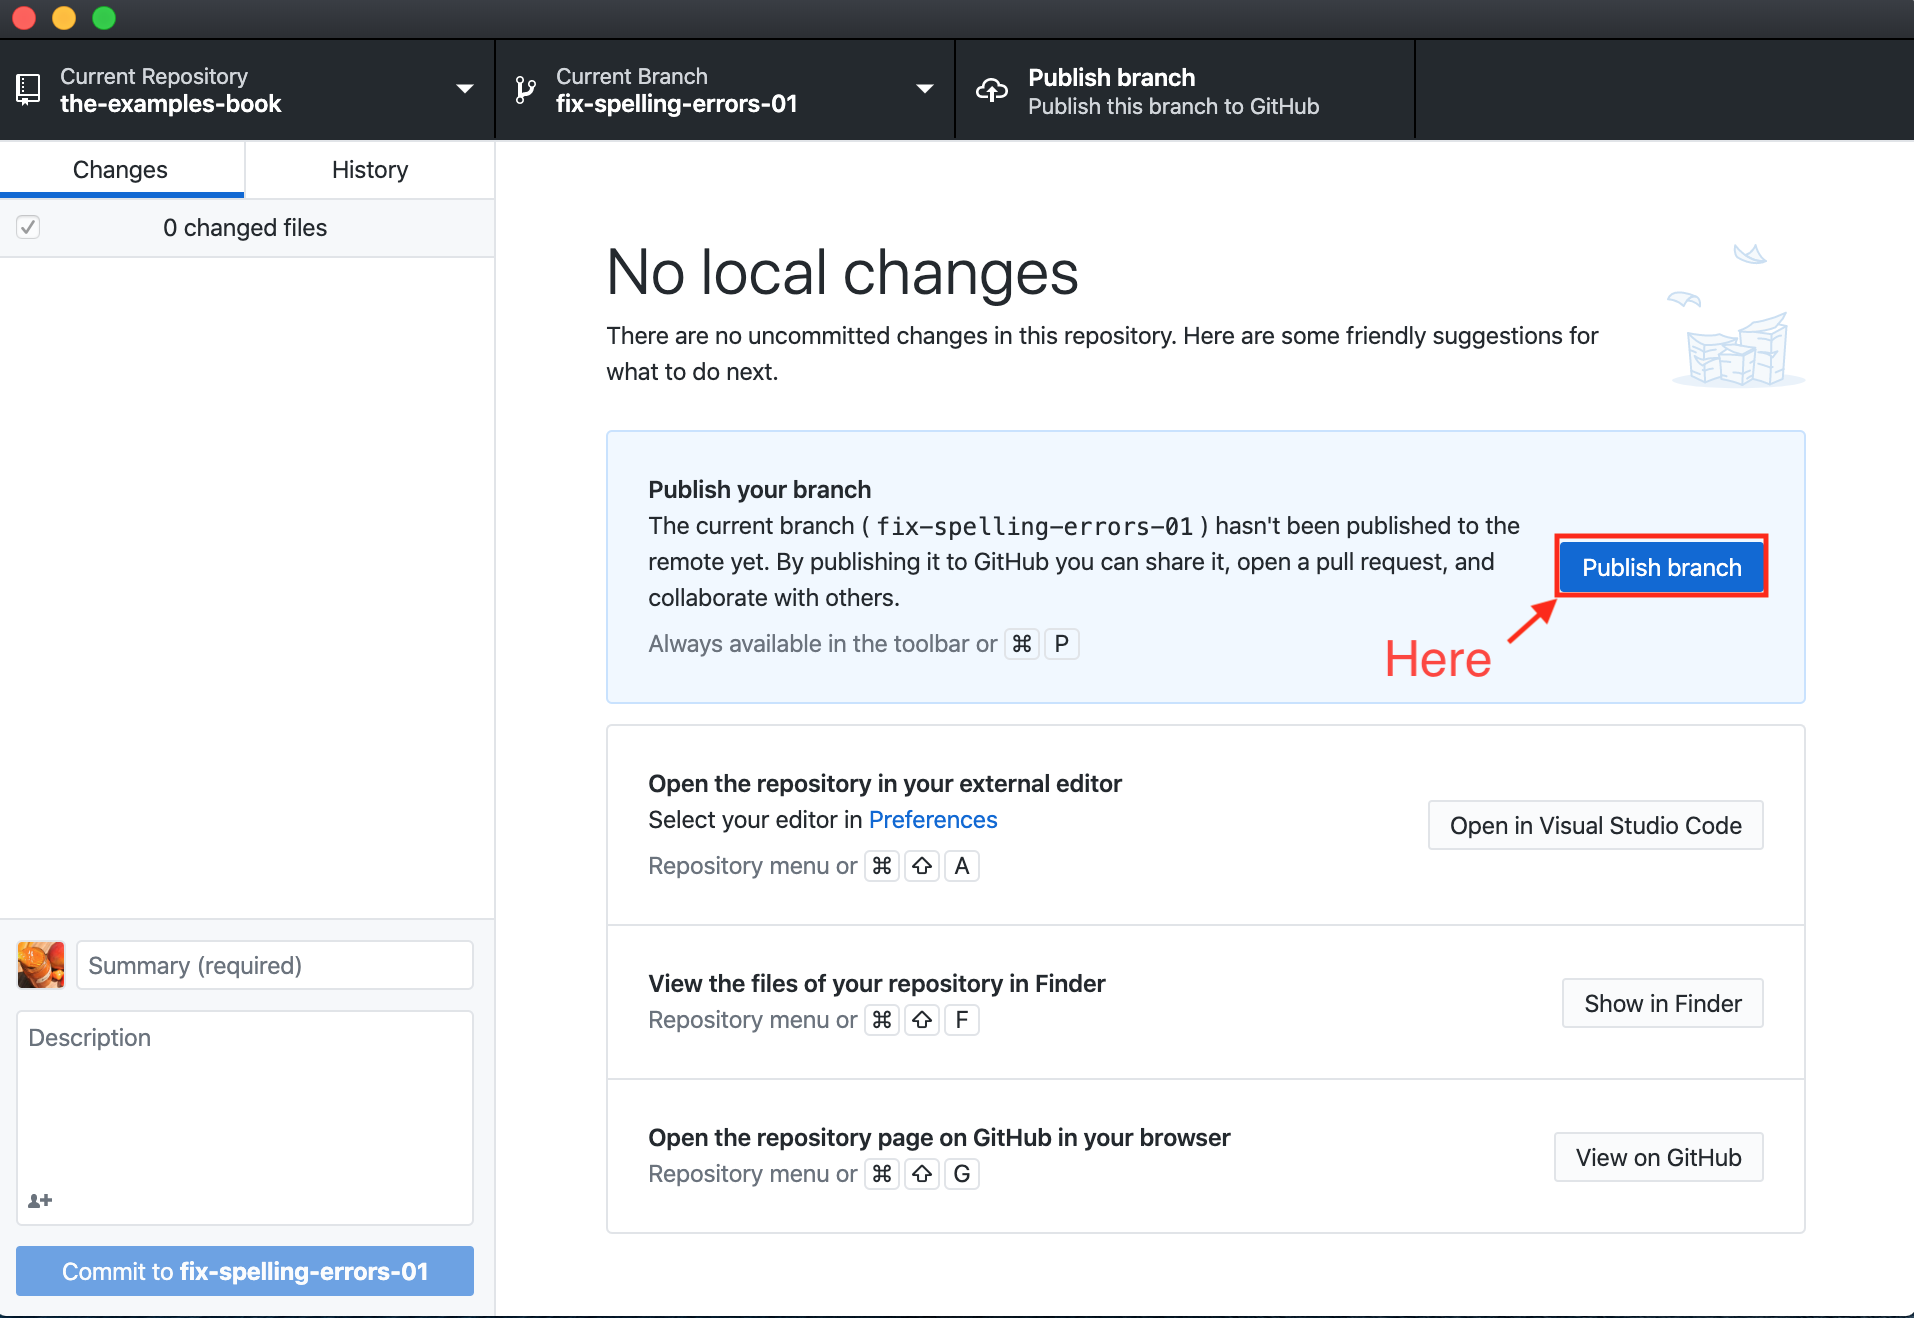
\includegraphics{./images/gh-desktop-13.png}
\caption{}
\end{figure}

\begin{enumerate}
\def\labelenumi{\arabic{enumi}.}
\setcounter{enumi}{18}
\tightlist
\item
  Upon publishing your branch, within GitHub Desktop, you'll be
  presented with the option to
  \protect\hyperlink{github-desktop-pull-request}{create a pull
  request}:
\end{enumerate}

\begin{figure}
\centering
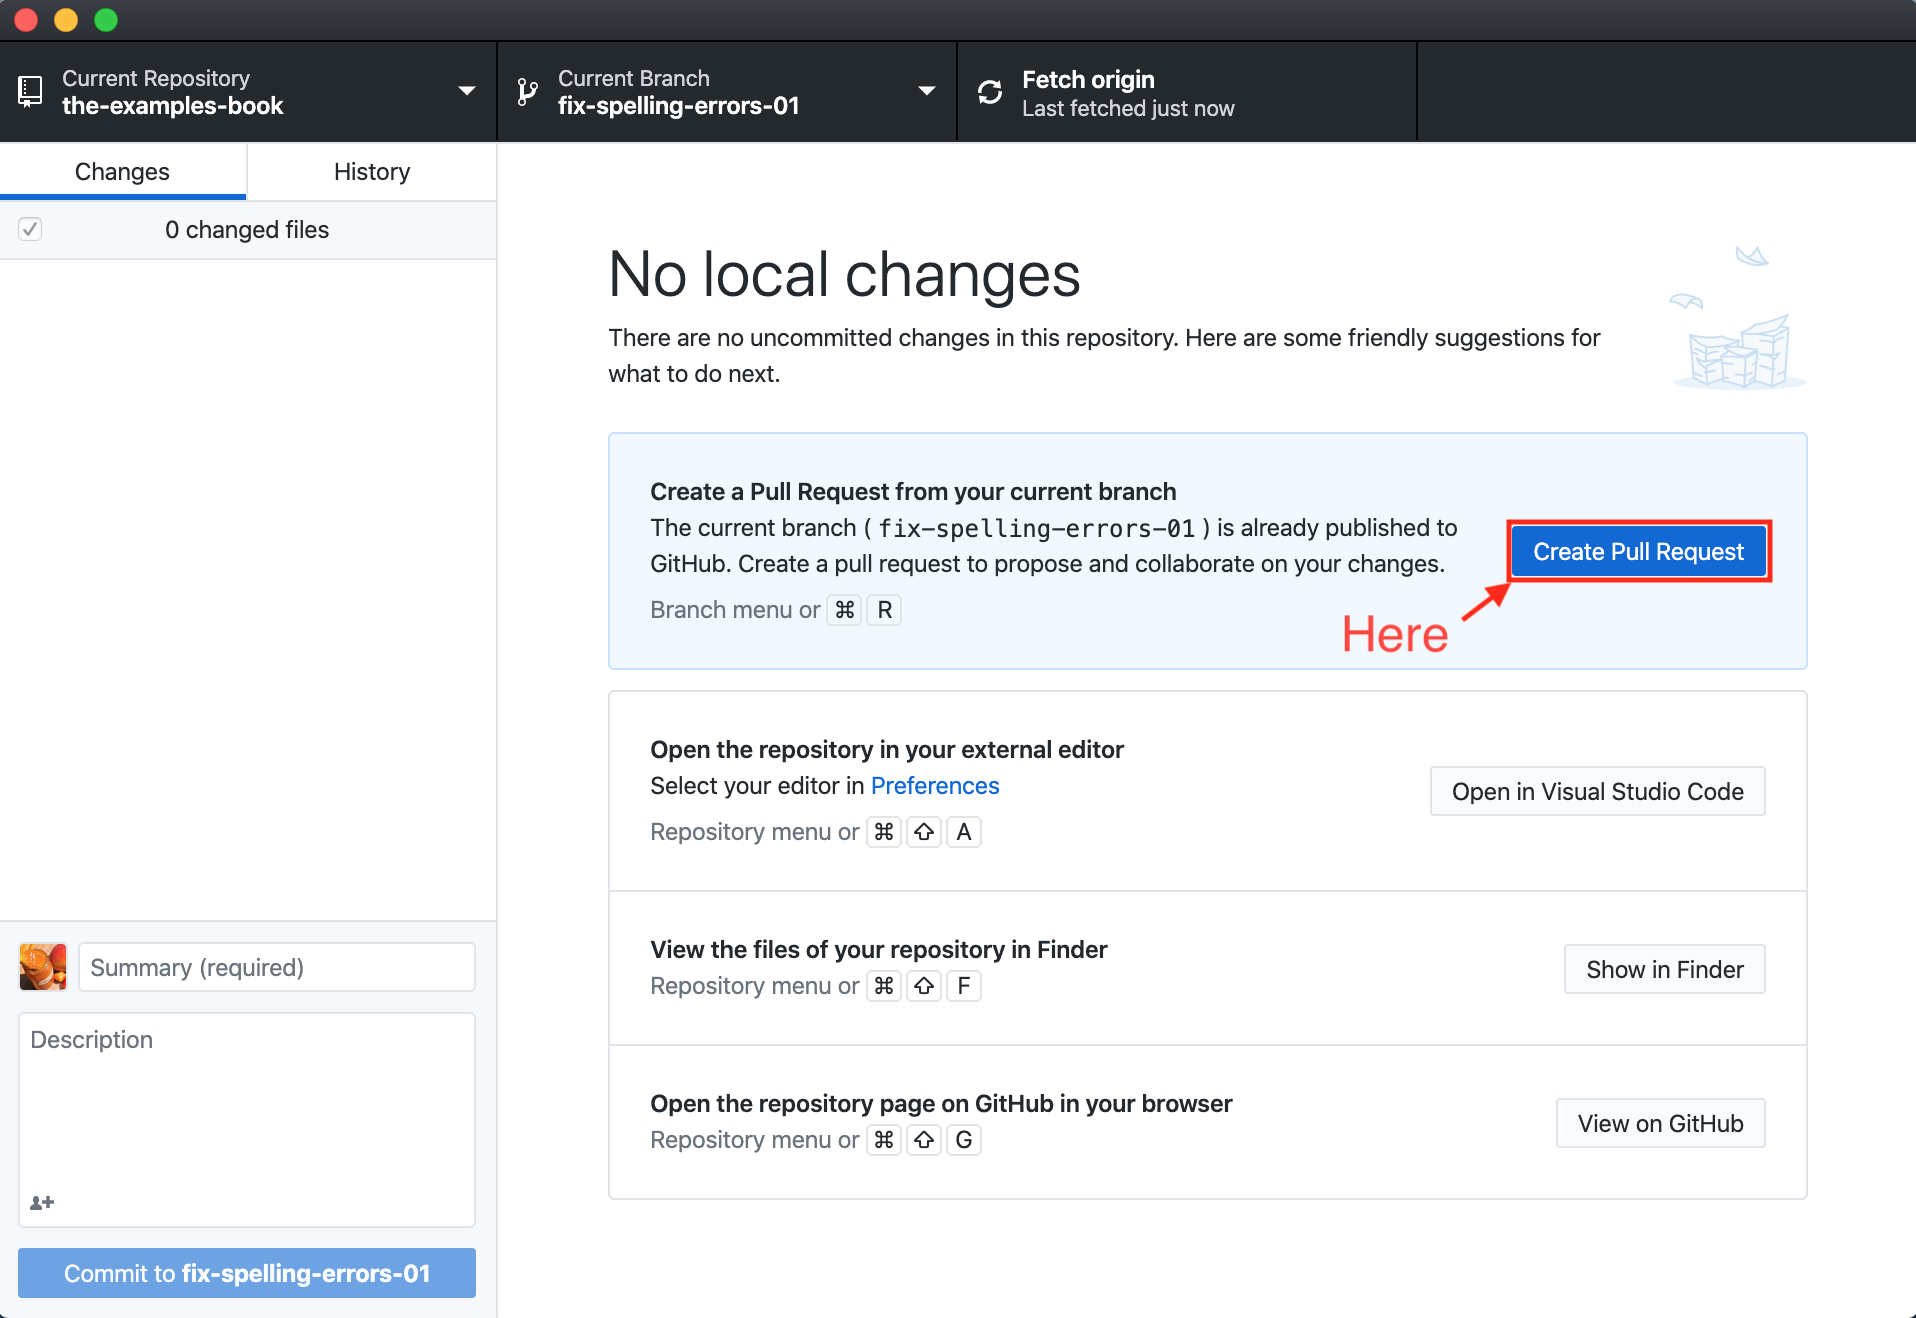
\includegraphics{./images/gh-desktop-12.png}
\caption{}
\end{figure}

\begin{enumerate}
\def\labelenumi{\arabic{enumi}.}
\setcounter{enumi}{19}
\tightlist
\item
  At this point in time, the repository owners will receive a
  notification and will check and potentially merge the changes into the
  \texttt{master} branch. © 2020 GitHub, Inc. Terms Privacy Security
  Status Help Contact GitHub Pricing API Training Blog About
\end{enumerate}

\chapter{Tips for Writing Great Documentation and
Walkthroughs}\label{tips-for-writing-great-documentation-and-walkthroughs}

\section{Find a Good Topic}\label{find-a-good-topic}

While writing documentation for a project, it would nearly impossible to
include every piece work completed or every line of code written. This
makes it important to pick important topics to write about. The goal is
to include as much specificty as possible while also remembering the
project as its entirety.

Here are a few helpful concepts to consider when choosing a topic:

\begin{enumerate}
\def\labelenumi{\arabic{enumi}.}
\item
  Step by step guides -- perfect for readers to learn quickly and
  implement in their own projects
\item
  In depth discussions of a specific topic -- great for readers who are
  looking for deeper knowledge in a topic
\item
  Numbered lists of useful facts about a common topic -- lightweight
  readings that readers can consume in bits and pieces.
\end{enumerate}

\section{Make Goals and Audience
Clear}\label{make-goals-and-audience-clear}

For these writings, our team will have a dual purpose of writing them.

\begin{enumerate}
\def\labelenumi{\arabic{enumi}.}
\item
  Record the work we have completed
\item
  Create a centralized location for tutorial based learning
\end{enumerate}

The audience to consider is future team members of the Merck-Data Mine
Corporate Partnership and Merck scientists looking to read and learn
from our work.

Remember to keep the audience and goal of our documentation in mind as
writing your entries.This will help the book keep continuiuty and give
readers the best chance to get exposed to the work that we have
completed.

\section{Have a Begining, Middle, and
End}\label{have-a-begining-middle-and-end}

It is important to have an introduction, body, and conclusion while
writing the documentation. This helps with fluidity within each document
and allows for easier comprehension.

\subsection{Introduction}\label{introduction}

The introduction should encourage the reader to continue reading. Start
with information about what will be covered in the read and how it
applies to the project. Try to keep the introduction less technical so
readers aren't discouraged by the complexity of the document.

\subsection{Body}\label{body}

The body is where you elaborate on all that you discussed in the
introduction. Provide depth and instruction while still relating to the
project as a whole. Use headings, photos, numbered lists, bullet points,
and formatting to help provide small bits of information at a time. This
is where you can facilitate a technical discussion with code.

\subsection{Conclusion}\label{conclusion}

Always finish the read with a conclusion, providing assurance of what
was just learned and include possible resources for more information
(i.e.~academic papers, blog posts, youtube videos). It is also
appropriate to give the reader a domain in which to use the skills they
have learned from your documentation.

\section{Getting Feedback and
Iterate}\label{getting-feedback-and-iterate}

Everyone on the team is encouraged to follow the documents that are
added to this book. Read through them and provide helpful feedback to
your teammate on how to improve.

Some common things to look out for:

\begin{enumerate}
\def\labelenumi{\arabic{enumi}.}
\item
  Formatting -- Does the document flow properly? Are there enough
  images, code, headers, etc\ldots{}?
\item
  Formality -- Is the document written well? Is the language approiate?
\item
  Goal and Audience -- Does the document relate to the goals and target
  audiences of this book?
\item
  Attention -- Was the reading interesting? Is there opportunity to
  learn from the read?
\end{enumerate}

\section{Practice, Practice, Practice}\label{practice-practice-practice}

Writing the entries in this book will undoubtably get better over time.
You are welcome to write as many entries as you'd like. They can be
simple or deep, long or short, imformational or technical, etc. As long
as the information in this book is informative and relevant to the
projects we hope to complete, it is encouraged for all members of the
team to write what they want!

\chapter{Documentation Example - The Basics of R
Markdown}\label{documentation-example---the-basics-of-r-markdown}

\section{Overview of R Markdown}\label{overview-of-r-markdown}

R Markdown is a file format for making dynamic documents with R. An R
Markdown document is written in markdown (an easy-to-write plain text
format) and contains chunks of embedded R code, text, images, headers,
and more.

In this walkthrough, we'll discuss some of the functionality of R
Markdown Documents and how to add images, code, and other features to
the document.

Throughout this tutorial, we'll be reviewing the contents of the R
Markdown cheat sheet that has most important information for writing in
Markdown. The cheat sheet can be found at
\url{https://rstudio.com/wp-content/uploads/2015/02/rmarkdown-cheatsheet.pdf}.

\section{Workflow}\label{workflow}

One of the great features of Markdown files is that they can be rendered
to PDF files, Word documents, HTML content, and more. This allows the
writer to easily write in R and export the document how they see best.

Take a look at a common lifecylce of R Markdown documents in th
following picture:

\begin{figure}
\centering
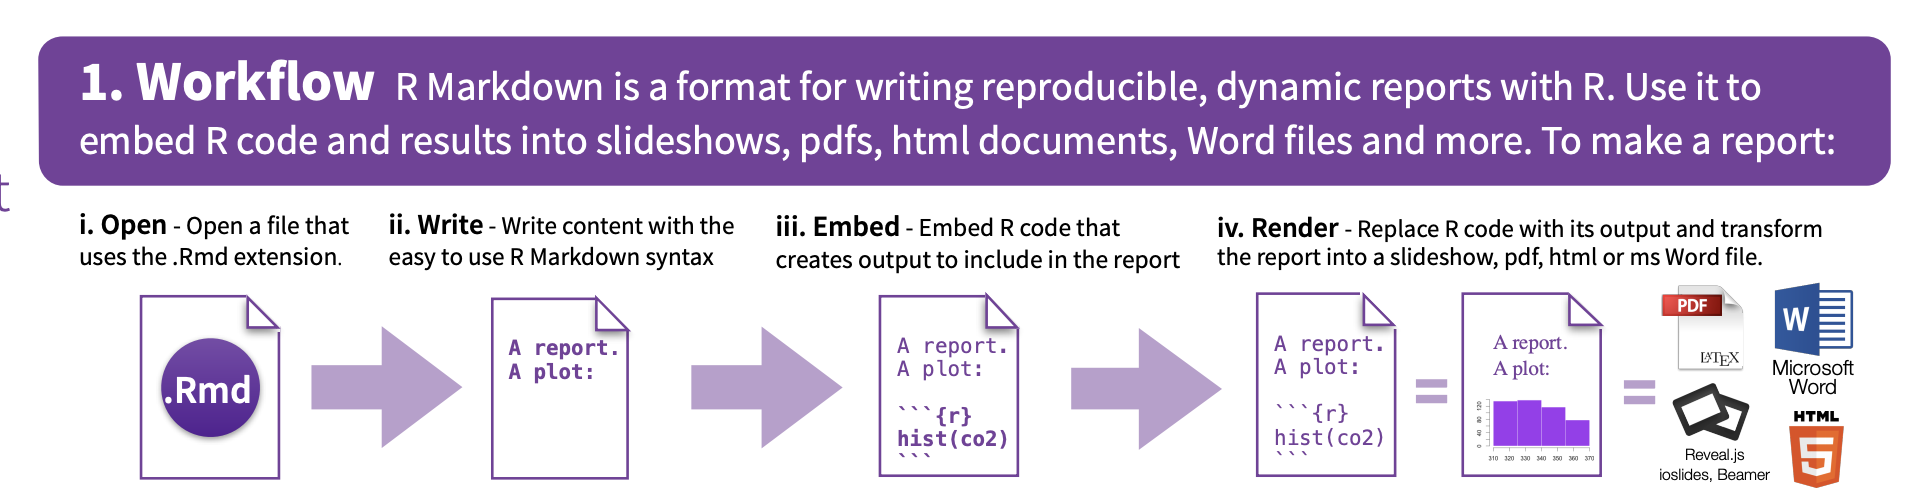
\includegraphics{images/workflow.png}
\caption{}
\end{figure}

\section{Opening a New File}\label{opening-a-new-file}

Writing R Markdown files is easiest within R Studio. Navigate to File
\textgreater{} New File \textgreater{} R Markdown to create a new file.

\begin{figure}
\centering
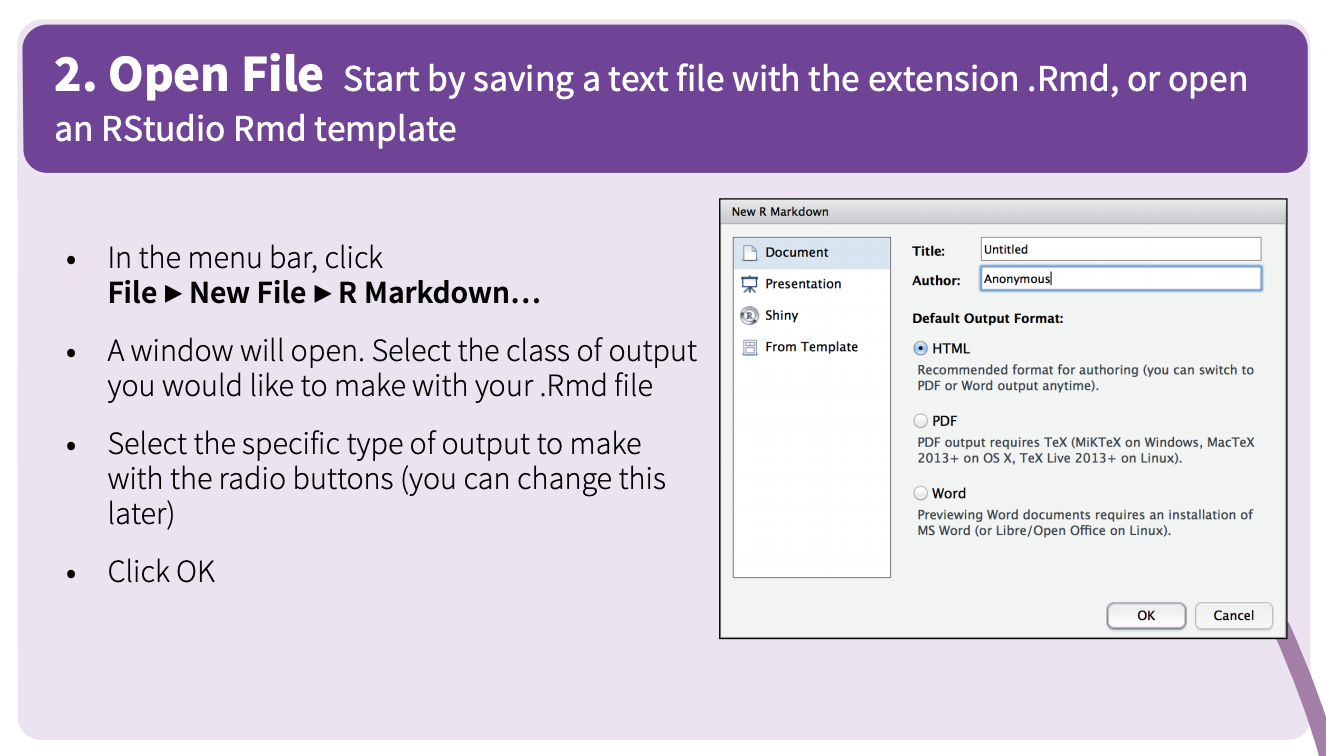
\includegraphics{images/open.png}
\caption{}
\end{figure}

\section{Helpful Syntax}\label{helpful-syntax}

Take a look through helpful sytax in this photo:

\begin{figure}
\centering
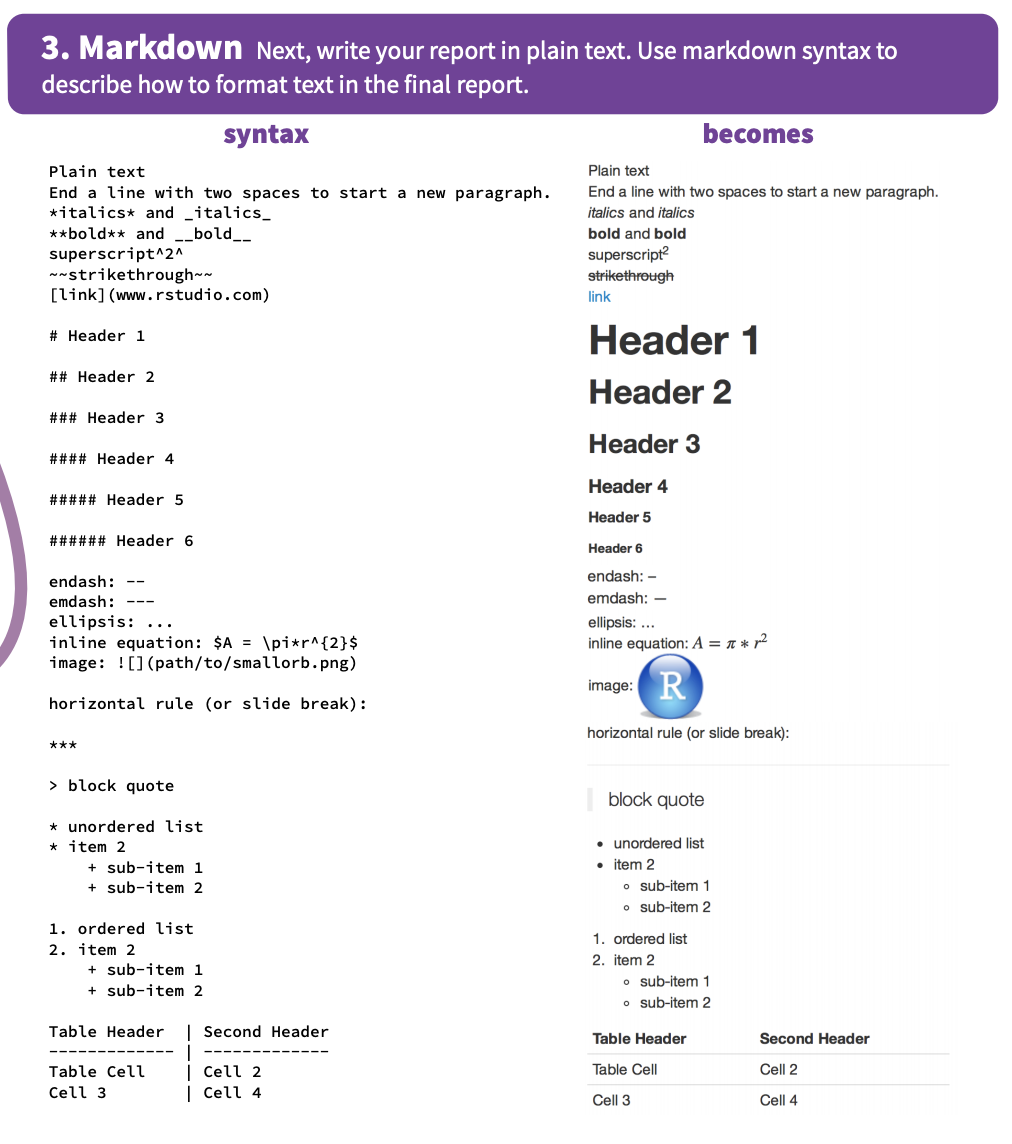
\includegraphics{images/syntax.png}
\caption{}
\end{figure}

Here are some examples to vie. Take a look at the raw R Markdown to view
the syntax in pratice.

\emph{italics} \textbf{bold} \sout{strikethrough}

\begin{quote}
Block Quote
\end{quote}

\begin{itemize}
\tightlist
\item
  Bullets
\item
  Bullets
\item
  subitem
\end{itemize}

\begin{enumerate}
\def\labelenumi{\arabic{enumi}.}
\tightlist
\item
  Lists
\item
  Lists
\end{enumerate}

\begin{itemize}
\tightlist
\item
  subitem
\end{itemize}

\section{Embed Code}\label{embed-code}

One of the best features of R Markdown is the ability to add code to
your document. To add a code snippet, click on the green \emph{insert}
button in your R Studio tool bar and choose which language you would
like to use!

\begin{Shaded}
\begin{Highlighting}[]
\KeywordTok{print}\NormalTok{(}\StringTok{"This is an R code snippet"}\NormalTok{)}
\end{Highlighting}
\end{Shaded}

\begin{verbatim}
## [1] "This is an R code snippet"
\end{verbatim}

\begin{Shaded}
\begin{Highlighting}[]
\BuiltInTok{print}\NormalTok{(}\StringTok{"This is a python code snippet with eval=FALSE"}\NormalTok{)}
\end{Highlighting}
\end{Shaded}

\begin{Shaded}
\begin{Highlighting}[]
\BuiltInTok{echo}\NormalTok{ this a bash code snippet}
\end{Highlighting}
\end{Shaded}

\begin{verbatim}
## this a bash code snippet
\end{verbatim}

\begin{figure}
\centering
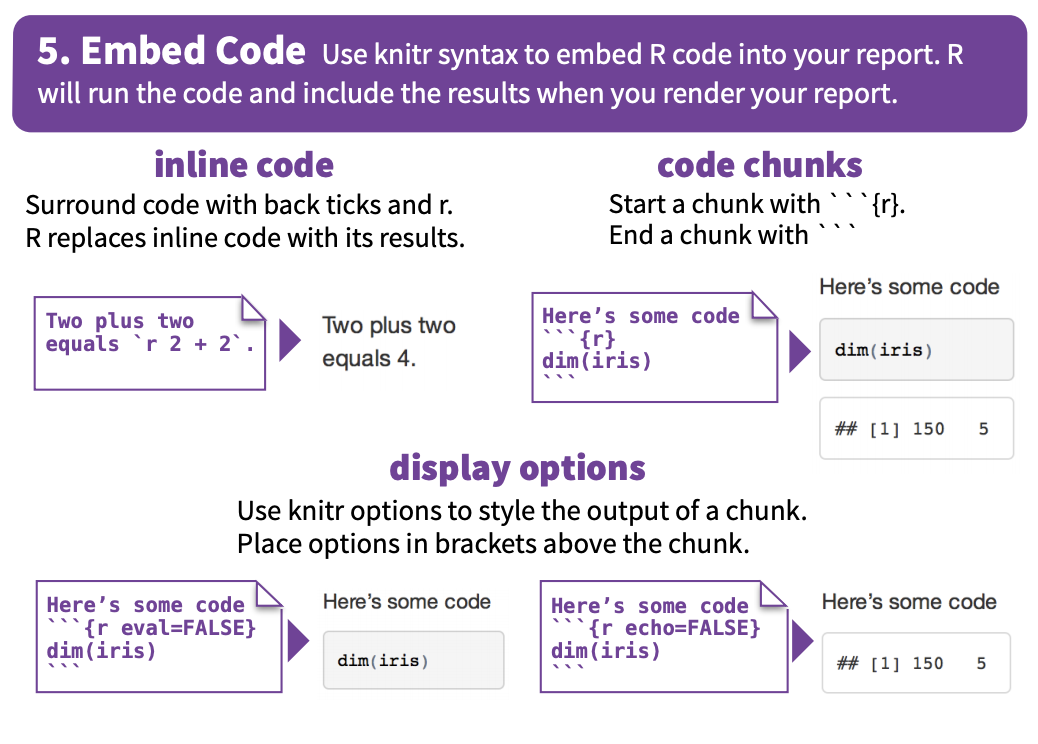
\includegraphics{images/code.png}
\caption{}
\end{figure}

There are also many options for your code snippets. Take a look:

\begin{figure}
\centering
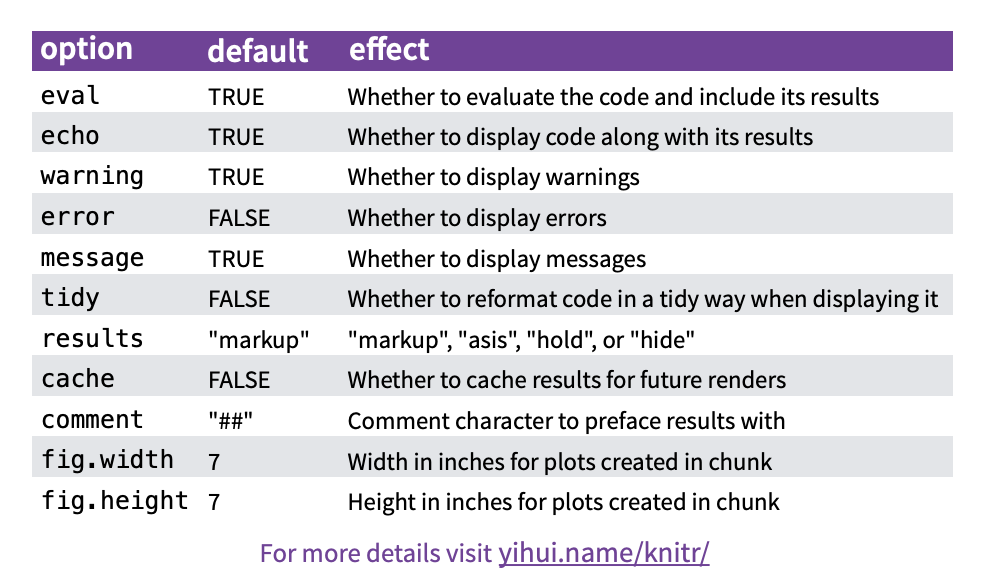
\includegraphics{images/options.png}
\caption{}
\end{figure}

\section{Wrapping (or knitting) it Up}\label{wrapping-or-knitting-it-up}

To knit your Markdown file you click the blue \emph{knit} button in your
R Studio toolbar. You can choose which file format you would like to
knit to as well!

For the purposes of our Merck-Data Mine documentation book, however, we
will not have to knit anything because we are placing the individual
documents in one bookdown book. To learn more about bookdown take a look
at \url{https://bookdown.org/yihui/bookdown/introduction.html} for more
information.

\chapter{Documentation Template}\label{documentation-template}

\section{Introduction}\label{introduction}

This section will give an overview of what was accomplished during the
previous sprint.

\section{Code}\label{code}

This section is where important code can be documented and commented on.
Some teams do not need to include all their code here as this would get
excessive. However, important functions or classes should be documented
and discussed here.

\section{Flow Diagrams /
Visualizations}\label{flow-diagrams-visualizations}

This is where teams should showcase flow diagrams of functions, data
pipeline, etc. This might also be a good place for
visualization/screenshots.

\section{White Paper}\label{white-paper}

When important decision are made, such as software specifications or
product developments, they should be documented in this section. Teams
should explain how they came to the conclusion and key takeaways about
the decision.

\section{Technical Report}\label{technical-report}

This section is where teams can highlight the processes of their work.
This is a more in depth look into what was accomplised during the sprint
where teams should describe step by step development.

\chapter{GitHub Test}\label{github-test}

This is to show changes in git.

\end{document}
